\chapter{Background}

\section{Automatic Drum Transcription}

As mentioned, \gls{ADT} describes the task of transcribing symbolic notation for drums from audio. To be even more descriptive, \gls{ADT} can be split into further tasks. From least to most complex we have: \gls{DSC}, where we classify drum instruments from isolated recordings. \gls{DTD}, where we transcribe audio containing exclusively drum instruments. \gls{DTP}, where we transcribe audio containing drum instruments, and additional percussive instruments which the transcription should exclude. Finally, we have \gls{DTM}, which describes the task of drum transcription with audio containing both drum, and melodic instruments.~\cite{8350302}

In this thesis, we will focus on the most complex of these, namely \gls{DTM}. Intuitively, we want to develop a deep learning model which, given input audio, has the ability to detect and classify different drum instrument onsets (events), while selectively ignoring unrelated, melodic instruments.

This task comes with difficulties not seen in the less complex tasks. Zehren et al.~\cite{signals4040042} describes one example, in where \textit{"melodic and percussive instruments can overlap and mask eachother..., or have similar sounds, thus creating confusion between instruments"}.

Even though deep learning has shown to be the most promising method to solve this task, different approaches has been tried, many with great success. Vogl et al.~\cite{vogl2018multiinstrumentdrumtranscription, Vogl2017DrumTV} showed good results with both a convolutional, and a convolutional-recurrent neural network. Zehren et al.~\cite{signals4040042, zehren2024analyzingreducingsynthetictorealtransfer} focused on datasets, showing that the amount of data and quality of data are equally important to get good performance. Most recently, Chang et al.~\cite{chang2024yourmt3multiinstrumentmusictranscription} explored an autoregressive, language model approach. This approach explored multi-instrument transcriptions, but their results on \gls{ADT} were notable.

This reinforces the fact that there still exist many approaches to attempt, which could lead to a general improvement on \gls{ADT} models.

\textcolor{red}{
Mention some more detailed background into \gls{ADT}, \gls{DTM}, etc.
Mention some more details into how it started, how it is going, etc.
Also why this is of interest. (Maybe also what is missing)
}

\textcolor{red}{
Mention the sequence to sequence prediction.
}

\section{Audio}

The US army~\cite{1953fundamentals} early described sound as \textit{"the sensation caused in the nervous system by vibration of the delicate membranes of the ear."}. In short, sound is the human perception of acoustic waves in a transition medium, like air. These waves, consisting of vibrating molecules, get picked up by our auditory organs and perceived by the brain. 

Thus sound can be described as the propogation and perception of waves. Mathematically, waves can be studied as signals~\cite{8454362}. To represent these sounds digitally, as \textit{audio}, one can express these waves as a signal, giving rise to the \textit{waveform}. The waveform is a representation of a signal as a graph, and charts the amplitude, or strength of the signal, over time.

\begin{figure}[H]
    \centering
    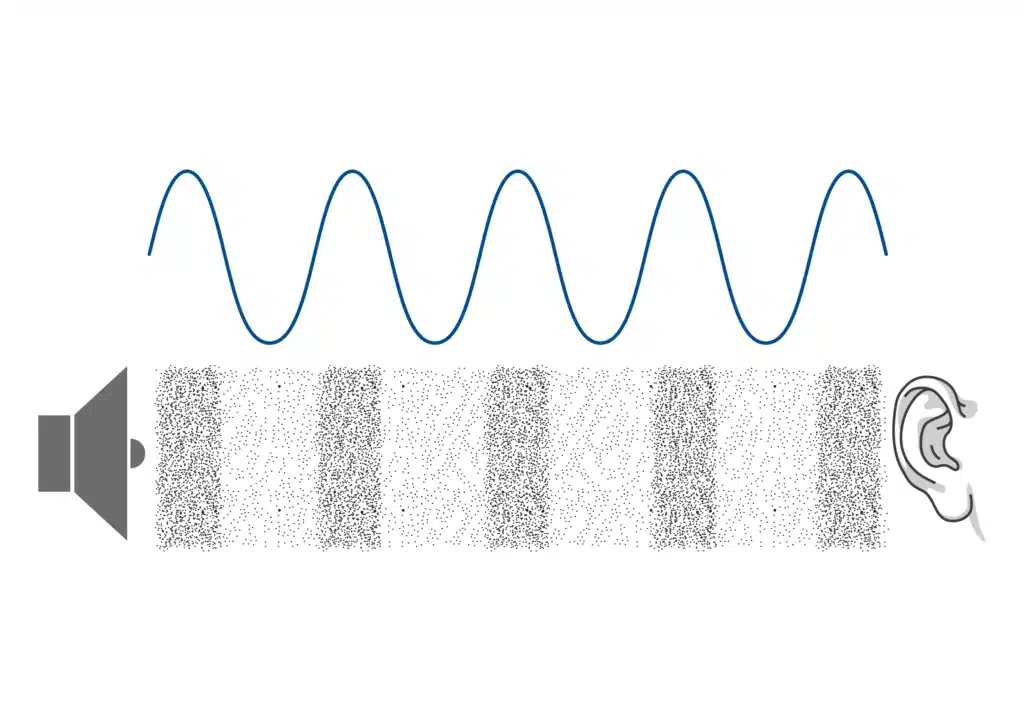
\includegraphics[scale=0.3]{figures/waveform}
    \caption{Soundwave to waveform relationship}
    \label{WaveformFigure}
\end{figure}

For monophonic sound, this waveform is a one-dimensional representation (in contrast to stereophonic, which is two-dimensional). Even though this is an excellent way of storing audio digitally, it is very compact. There have been deep learning models working directly with these waveforms, e.g. Oord et al.'s WaveNet~\cite{oord2016wavenetgenerativemodelraw}, however the task of just parsing and perceiving such a signal is a complex one.

\subsection{Fourier Transform}

By utilising the fact that 